\documentclass[12pt, hyperref={bookmarks=false}, show notes]{beamer}
% Text
	\usepackage[T1]{fontenc}
	\usepackage[utf8]{inputenc}
	\usepackage[english]{babel}
	% \usepackage[bitstream-charter]{mathdesign} % Serif font (Charter BT).
	\usepackage[scaled=0.84]{DejaVuSansMono} % Monospaced font.
	\def\sfdefault{SourceSansPro-TLF} % Sans serif font.
	\usepackage{textcomp}

% Maths
  \usepackage{amsmath}
  \usepackage{mathtools}
  \usepackage{siunitx}
  % Vector command
  \newcommand{\omatrix}[1]{\ensuremath{\boldsymbol{#1}}}

% Graphics
  \usepackage{graphicx}
  \usepackage[caption=false]{subfig}
	\usepackage{tikz}
  \usepackage{pgfplots}
  \pgfplotsset{compat=1.10}
	% ADD TIKZ LIBRARIES
  \usetikzlibrary{calc}
  \usetikzlibrary{arrows.meta}
  %\usepackage{tikz-qtree}
  \usetikzlibrary{decorations.pathmorphing}
  \usetikzlibrary{matrix,shapes,positioning}
  \usepgfplotslibrary{external}
  \tikzexternalize[prefix=gfx/tikz/]
  %\tikzexternaldisable % Disable by default
  \usepackage{pgfgantt}
  \usepackage{mdframed}
  \newmdenv [align=center, backgroundcolor=color3!10, linecolor=color3!50, linewidth=1pt]{mtjbox}

	\usepackage{xcolor}
    \definecolor{color1}{cmyk}{100,50,0,0}   % blue
    \definecolor{color2}{cmyk}{0,80,100,0}   % vermillion
    \definecolor{color3}{cmyk}{97,0,75,0}    % blueish green
    \definecolor{color4}{RGB}{204,121,167}    % reddish purple
    \definecolor{color5}{RGB}{230,159,0}   % orange
    \usepackage{colortbl}
% Misc
\usepackage{booktabs}
\usepackage{enumerate}
\usepackage{pdfpages}
\usepackage{pgfpages}
\usepackage{setspace}
%\usepackage{multimedia}

% Box colors.
\definecolor{clframe}{gray}{0.75}
\definecolor{clshade}{gray}{0.95}
\definecolor{clcodeshade}{gray}{0.93}

% Code colors.
\definecolor{javared}{rgb}{0.6,0,0}            % for strings
\definecolor{javagreen}{rgb}{0.25,0.5,0.35}    % comments
\definecolor{javapurple}{rgb}{0.6,0,0.5}       % keywords
\definecolor{javadocblue}{rgb}{0.25,0.35,0.75} % javadoc

\usepackage{listings}

\lstdefinestyle{javastyle}{%
  language=Java,
  keywordstyle=\color{javapurple}\bfseries,
  stringstyle=\color{javared},
  commentstyle=\color{javagreen},
  morecomment=[s][\color{javadocblue}]{/**}{*/}
}

\lstnewenvironment{javacode}[1][]{%
  \lstset{style=javastyle, #1}
}{}

\lstset{
  columns=flexible,
  escapechar=",
  escapeinside={(*@}{@*)},
  basicstyle=\ttfamily\footnotesize,
  frame=single, backgroundcolor=\color{clshade}, rulecolor=\color{clframe},
  framerule=\fboxrule, xleftmargin=3.4pt, xrightmargin=3.4pt, belowskip=\smallskipamount,
  captionpos=b,
  numbers=left,
  numberstyle=\scriptsize,
  numbersep=7pt,
  tabsize=2,
  keepspaces=true,
  showspaces=false,
  showstringspaces=false,
  breaklines=true,
  breakatwhitespace=true,
  postbreak=\raisebox{0ex}[0ex][0ex]{\ensuremath{\color{red}\hookrightarrow\space}}
}

\setbeamertemplate{navigation symbols}{}
%\setbeamertemplate{bibliography item}[text]

%\usepackage{caption}
\usetheme{/amsterdam}
\date{January 21, 2015}

\usepackage{beamertheme/handoutWithNotes}
% Uncomment for handouts. Add \documentclass[12pt,handout]{beamer}
%\pgfpagesuselayout{4 on 1 with notes}[a4paper,border shrink=5mm]
% Comment for handouts.
\setbeameroption{show notes on second screen=right}

% Table of content dybde (0-index)
%\setcounter{tocdepth}{1}

% BibLaTeX
%\usepackage{csquotes}
%\usepackage[
%backend=bibtex,
%citestyle=numeric,
%bibstyle=numeric,
%maxcitenames=3,
%maxbibnames=99,
%url=true]{biblatex}
%\addbibresource{../rapport/references/refs.bib}
%\addbibresource{extrasources.bib}
%\usepackage{../style/biblatex_custom_formatting}

\graphicspath{{gfx/}{../report/graphics/}{../report/graphics/tikz}}

\begin{document}

%\captionsetup[figure]{font=small,singlelinecheck=off,justification=raggedright}

\title[Adapting and Implementing Continuous Integration Principles and Scrum]{Adapting and Implementing Continuous Integration Principles and Scrum}
% \author[\insertframenumber /\inserttotalframenumber]{sw609f15}
\makeatletter
  \defbeamertemplate*{footline}{myminiframes theme}
  {%
    \begin{beamercolorbox}[colsep=1.5pt]{upper separation line foot}
    \end{beamercolorbox}
    \hbox{%
      \begin{beamercolorbox}[wd=.75\paperwidth,ht=2.5ex,dp=1.125ex,%
        leftskip=.3cm,rightskip=.3cm plus1fil]{title in head/foot}%
        \leavevmode{\usebeamerfont{title in head/foot}\insertshorttitle}%
      \end{beamercolorbox}%
      \begin{beamercolorbox}[wd=.15\paperwidth,ht=2.5ex,dp=1.125ex,%
        leftskip=.3cm,rightskip=.3cm]{title in head/foot}%
        {\usebeamerfont{author in head/foot}\usebeamercolor[fg]{author in head/foot}\insertshortauthor}
      \end{beamercolorbox}%
      \begin{beamercolorbox}[wd=.1\paperwidth,ht=2.5ex,dp=1.125ex,%
        leftskip=.3cm,rightskip=.3cm,center]{title in head/foot}%
        {\usebeamerfont{author in head/foot}\usebeamercolor[fg]{author in head/foot}\insertframenumber/\inserttotalframenumber}%
      \end{beamercolorbox}%
    }%
    \begin{beamercolorbox}[colsep=1.5pt]{lower separation line foot}
    \end{beamercolorbox}
  }
\makeatother

% Adding front slide.
{
\setbeamercolor{background canvas}{bg=}

\includepdf[pages=1]{frontslide.pdf}
}

\begin{frame}
  \frametitle{Indhold}
  \tableofcontents
  \note{
  \begin{itemize}
    \item Noter...
  \end{itemize}
}
\end{frame}


%\chapter{Introduction}
\kimnote{Et projekt skal starte med en general forklaring af problemstillingen i den virklige verden. Derefter kan i nævne formelle ting.}
The purpose of this semester project is to develop a complex software system in a large development environment. The software system is called GIRAF (Graphical Interface Resources for Autistic Folk) and is inherited from the 6\textsuperscript{th} semester students of past years. The project is a collaboration between Aalborg University, Aalborg Municipality and several institutions that work with autistic citizens. 
\kimnote{I skal beskrive hvem der præcis er jeres kunder og ikke bare nogle af dem. Det er nok bedst er flytte sådan en redegørelse et andet sted hen.}

The GIRAF project was initiated by Ulrik Nyman, Associate Professor at Aalborg University, in 2011. It is a software suite aimed at easing the daily routines of autistic citizens and their guardians. Autistic citizens generally have limited language skills and thus their primary way of communicating is through pictograms. An important aspect of the multi-project is therefore easing this communication.

Most are Android apps.
The project consists of several front-end and back-end subprojects, that each serves a purpose of the combined system. Most of the Examples of the subprojects are \todo{Insert example applications with brief description}.

\begin{description}
  \item[Launcher] \dummy
  \item[Sekvens]
  \item[Pictooplæser]
	\item[Kategoriværktøjet] \dummy
  \item[Picto Creator] Hvad er dette?
  \item[Pictotegner]
  \item[Picto Search] \dummy
  \item[Oasis App]
  \item[Ugeplan]
  \item[Tidstager] 
  \item[Stemmespillet]
  \item[Kategorispillet]
  \item[Web Ugeplan]
  \item[Webadmin]
\end{description}
\todo{This list are the front-end apps. Maybe move to appendix?}
\kimnote{Forklar det der er essentielt for jeres projekt. Det kunne være fint med en liste over de andre "projekter" i appendix, men brug kun tid på det hvis det bringer værdi til jeres projekt. Det der skal stå i en rapport er hvad i har lavet krydret en passende mængde context.}

There are 14 project groups with approximately 4 students in each. It is crucial that project groups work towards creating a working system, and to allow this a common work process has been decided by the semester coordinator. As such, the semester is split into four sprints (in Scrum terms). \kimnote{I bør introducere jeres process(scrum) før i begynder at bruge fagtermer fra den. Det er nok med et par linjer her i intruduktionen hvor i skriver at i bruger scrum. Jeg tror det vil gavne jer at have en kort sektion om jeres adoptering af scrum, altså hvilke scrum værktøjer i bruger, medmindre i bruger ren scrum!}
The organization of this report reflects these sprints. \todo{Write more about early process decisions.}

\begin{documentorganization}
  \item In \chapterref{chap:sw_dev_method} we describe the software development method used across the multi-project as well as in our group;
  \item Sprint 0:
  \begin{itemize}
    
    \item In \chapterref{chap:sprint1_planning} we describe the sprint planning process;
    \item In \chapterref{chap:config_management} we describe our responsibility as the configuration management group;
    \item In \chapterref{chap:sprint1_end} we describe and conclude on the sprint. 
  \end{itemize}
  \item Sprint 1:
  \begin{itemize}
    \item \todo{Fill Sprint 1 content in.}
  \end{itemize}
  \item Sprint 2:
  \begin{itemize}
    \item \todo{Fill Sprint 2 content in.}
  \end{itemize}
  \item Sprint 3:
  \begin{itemize}
    \item \todo{Fill Sprint 3 content in.}
  \end{itemize}
\end{documentorganization}

\todo{Skriv noget om ``external customer'' da vi også har ``internal customers''}
\section[Udviklingsmetode]{Udviklingsmetode}

% Emneoverskrift. Start jeres del med denne:
\begin{frame}
  \frametitle{}
  \begin{center}
    {\Huge Udviklingsmetode}
  \end{center}
\end{frame}
\note{
  \begin{itemize}
		\item Notes...
  \end{itemize}
}

\begin{frame}
    \frametitle{Udviklingsmetode i multiprojektet}
    \centering
    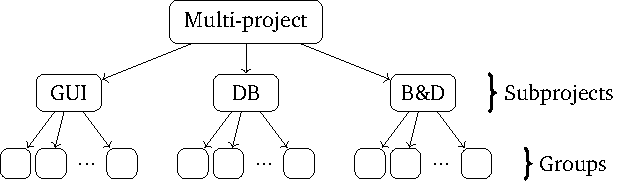
\includegraphics[width=0.8\textwidth]{multiproject_illustration.pdf}
\end{frame}
\note{
	\begin{itemize}
    \item \textbf{Unik struktur}. Vi ønsker at \textbf{tilfredsstille} kunden, men har også andre \textbf{prioriteter} såsom gode, indholdsrige emner, så \textbf{rapport} og \textbf{karakter} bliver gode.
    \item Vi kan ikke \textbf{fyre }grupper, \textbf{ingen autoritet}.
    \item Vi har valgt: \textbf{Scrum of Scrums} i 3 niveauer
    \item \textbf{AGIL} METODE godt valg:
    \begin{itemize}
      \item ingen \textbf{udvikler-erfaring} med kode + krav + kunder
      \item \textbf{Kun 4 måneder} > ikke tid til at forstå kodebasen
      \item Vi skal bruge tiden på at få den til at virke!
    \end{itemize}
    \item Scrum ca. 7 mand. \textbf{2 niveauer}: 15 mand
    \begin{itemize}
      \item Multiprojekt: Sikre at roller, work products og møderne overholdes.
      \item Subprojekt: Sprint planning, sprint review, og internt løse større problemer.
      \item Gruppe: Scrum of (something). Grupperne skal implementere interfacet Scrum. Samarbejde user stories input, estimering mm.
    \end{itemize}
	\end{itemize}
}

\begin{frame}
    \frametitle{Udviklingsmetode i multiprojektet}
    \framesubtitle{Typer af backlog items}
      \begin{mtjbox}[backgroundcolor=color1!5, linecolor=color1!40]
        Backlog Items
        \begin{columns}
          \begin{column}{0.48\textwidth}
            \begin{mtjbox}
              Feature (+ bug)
            \end{mtjbox}
          \end{column}
          \begin{column}{0.48\textwidth}
            \begin{mtjbox}
              Constraint
            \end{mtjbox}
          \end{column}
        \end{columns}

        \begin{columns}
          \begin{column}{0.48\textwidth}
            \begin{mtjbox}
              Knowledge Acquisition
            \end{mtjbox}
          \end{column}
          \begin{column}{0.48\textwidth}
            \begin{mtjbox}
              Technical Work
            \end{mtjbox}
          \end{column}
        \end{columns}
      \end{mtjbox}

\end{frame}
\note{
	\begin{itemize}
    \item \textbf{Vi startede} med 1 type: USER STORIES
    \item Kritik fra en anden gruppe: Svært at formulere, prioritere og arbejde på technical work, og knowledge acquisition.
    \item \textbf{Revidering}, databasegrupperne (technical work)
    \item \textbf{Feature/bug}: funktionelle krav, værdi for kunden.
    \item \textbf{Constraint}: non-funktionelle krav, ikke tvinge ind i user story. Skrives på bagside, eller egen post-it.
    \item \textbf{Knowledge Acquisition}: Undersøge ting. Timeboxing muligt: spike fra XP.
    \item \textbf{Technical Work}: Vigtige opgaver for os udviklere (system+refactoring).

	\end{itemize}
}

\begin{frame}
    \frametitle{Udviklingsmetode i multiprojektet}
    \centering
    \StickyNoteFront{\ECFAugie{} \small As a <\emph{type of user}>,\\I want <\emph{some goal}>\\so that <\emph{some reason}>}
    ~~~~~~~
    \StickyNoteBack{\ECFAugie{} \small Conditions of satisfaction} % for sjov font
\end{frame}
\note{
  \begin{itemize}
    \item Før havde vi ikke en fast måde at skrive user stories.
    \item Revidering:
    \item Formulering konsekvent: nemmere at sammenligne, mere sigende.
    \item As a <type of user>, I want <some goal> so that <some reason>.
    \begin{itemize}
      \item ``type of user'' kan være udvikler, slutbruger eller andet.
    \end{itemize}
  \end{itemize}
}

\begin{frame}
    \note{
      \begin{itemize}
        \item Scrum master: \textbf{os}, som følge af \textbf{ansvar} for udviklingsmetode.
        \begin{itemize}
          \item Scrum Master for alle projektgrupper.
          \item \textbf{Overser metoder}
          \item \textbf{Guider} grupperne til at følge Scrum
        \end{itemize}
        \item Product owner: Skal \textbf{kende kundernes behov}, kontakt med kunder.
        \begin{itemize}
          \item \textbf{I starten}: 1 sprint review møde med eksterne kunder.
          \item Semesterkoordinator: kunderne er \textbf{ligeglade} med interne ting.
          \item \textbf{Løsning}: 3 sprint reviews. GUI speciel (kunde)
          \item I den forbindelse overvejede vi noget af \textbf{strukturen} i Scrum-of-Scrums.
          \item \textbf{Løsning}: Et subprojekt har egen product owner, kunde og backlog.
          \item ~~~~ Grupper kan være kunder for grupper.
          \item Figur: GUI har eksterne kunder som kunder. Resten har GUI og hinanden som kunder.
        \end{itemize}
      \end{itemize}
    }
    \frametitle{Udviklingsmetode i multiprojektet}
    \framesubtitle{Roller}
    \begin{columns}[t]
    \column{.5\textwidth}
      \begin{mdframed}[align=center, backgroundcolor=color3!10, linecolor=color3!50, linewidth=1pt]
        Scrum Master
      \end{mdframed}
    \column{.5\textwidth}
      \begin{mdframed}[align=center, backgroundcolor=color3!10, linecolor=color3!50, linewidth=1pt]
        Product Owner
      \end{mdframed}
      \vspace{.6cm}
      \centering
      \pause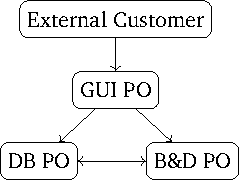
\includegraphics[width=.65\textwidth]{po_illustration.pdf}
    \end{columns}
\end{frame}



% Indhold:
\begin{frame}
    \frametitle{Udviklingsmetode i vores gruppe}
    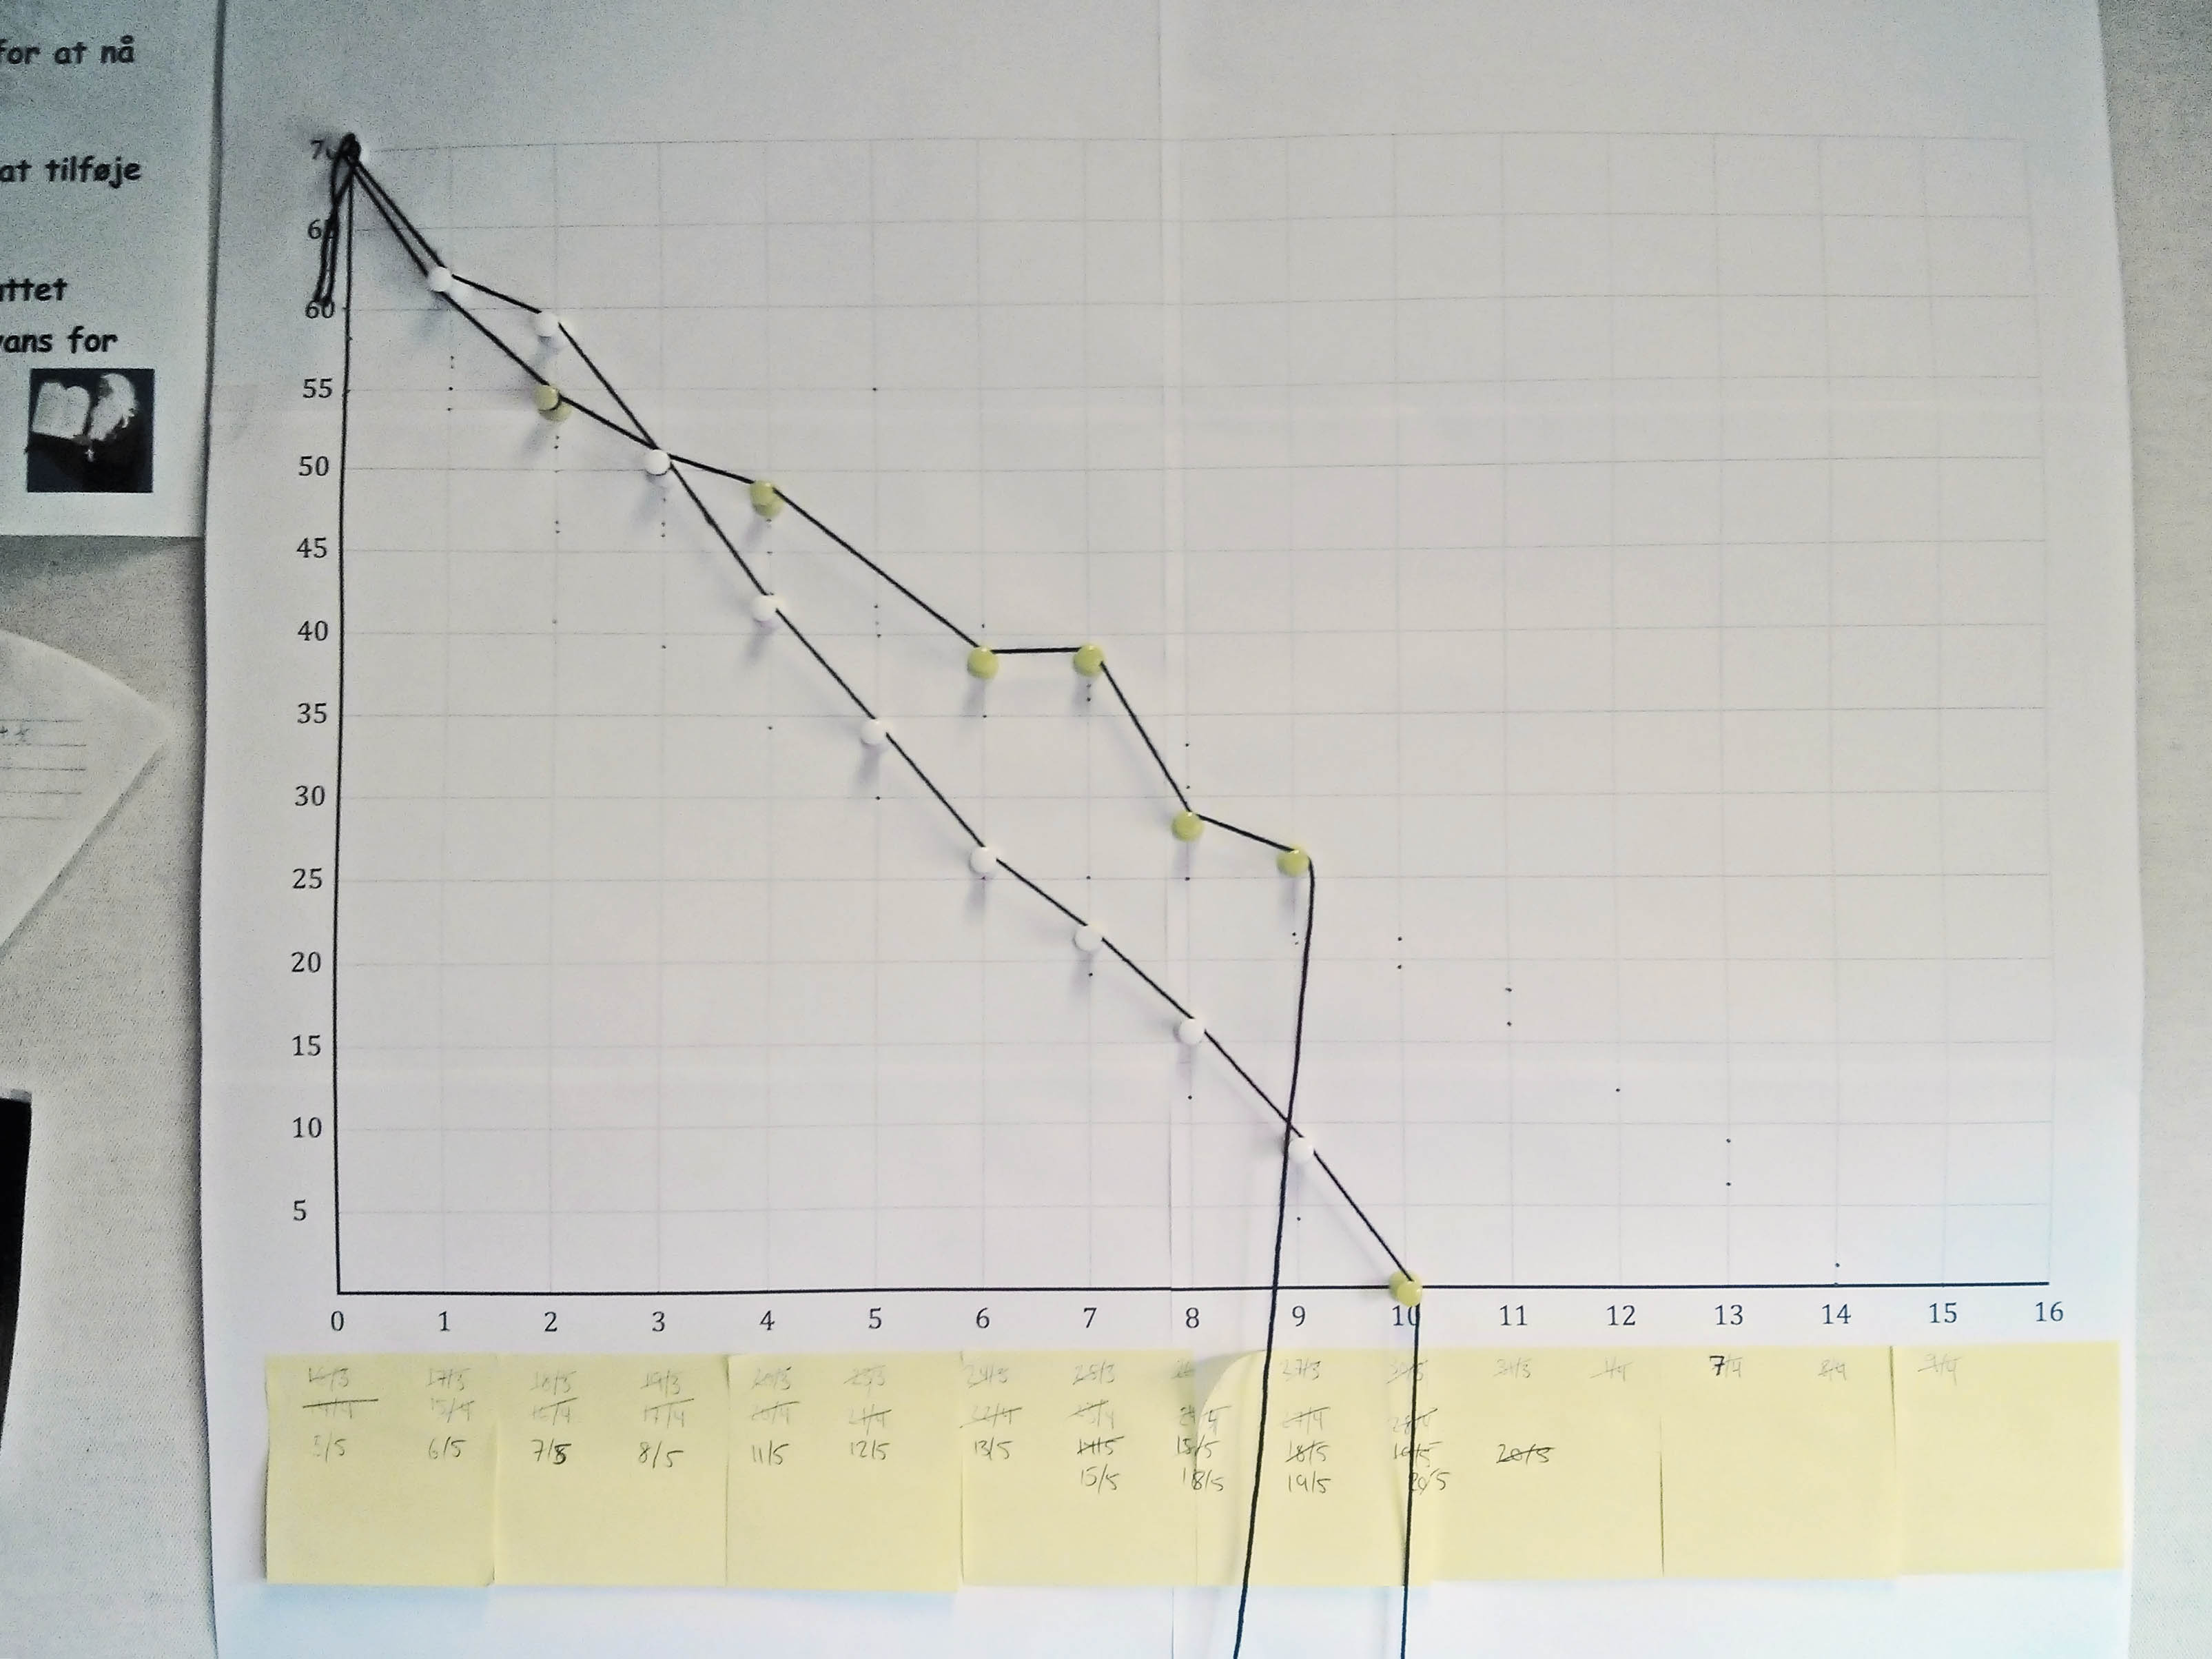
\includegraphics[width=0.49\textwidth]{burndown}~~~
    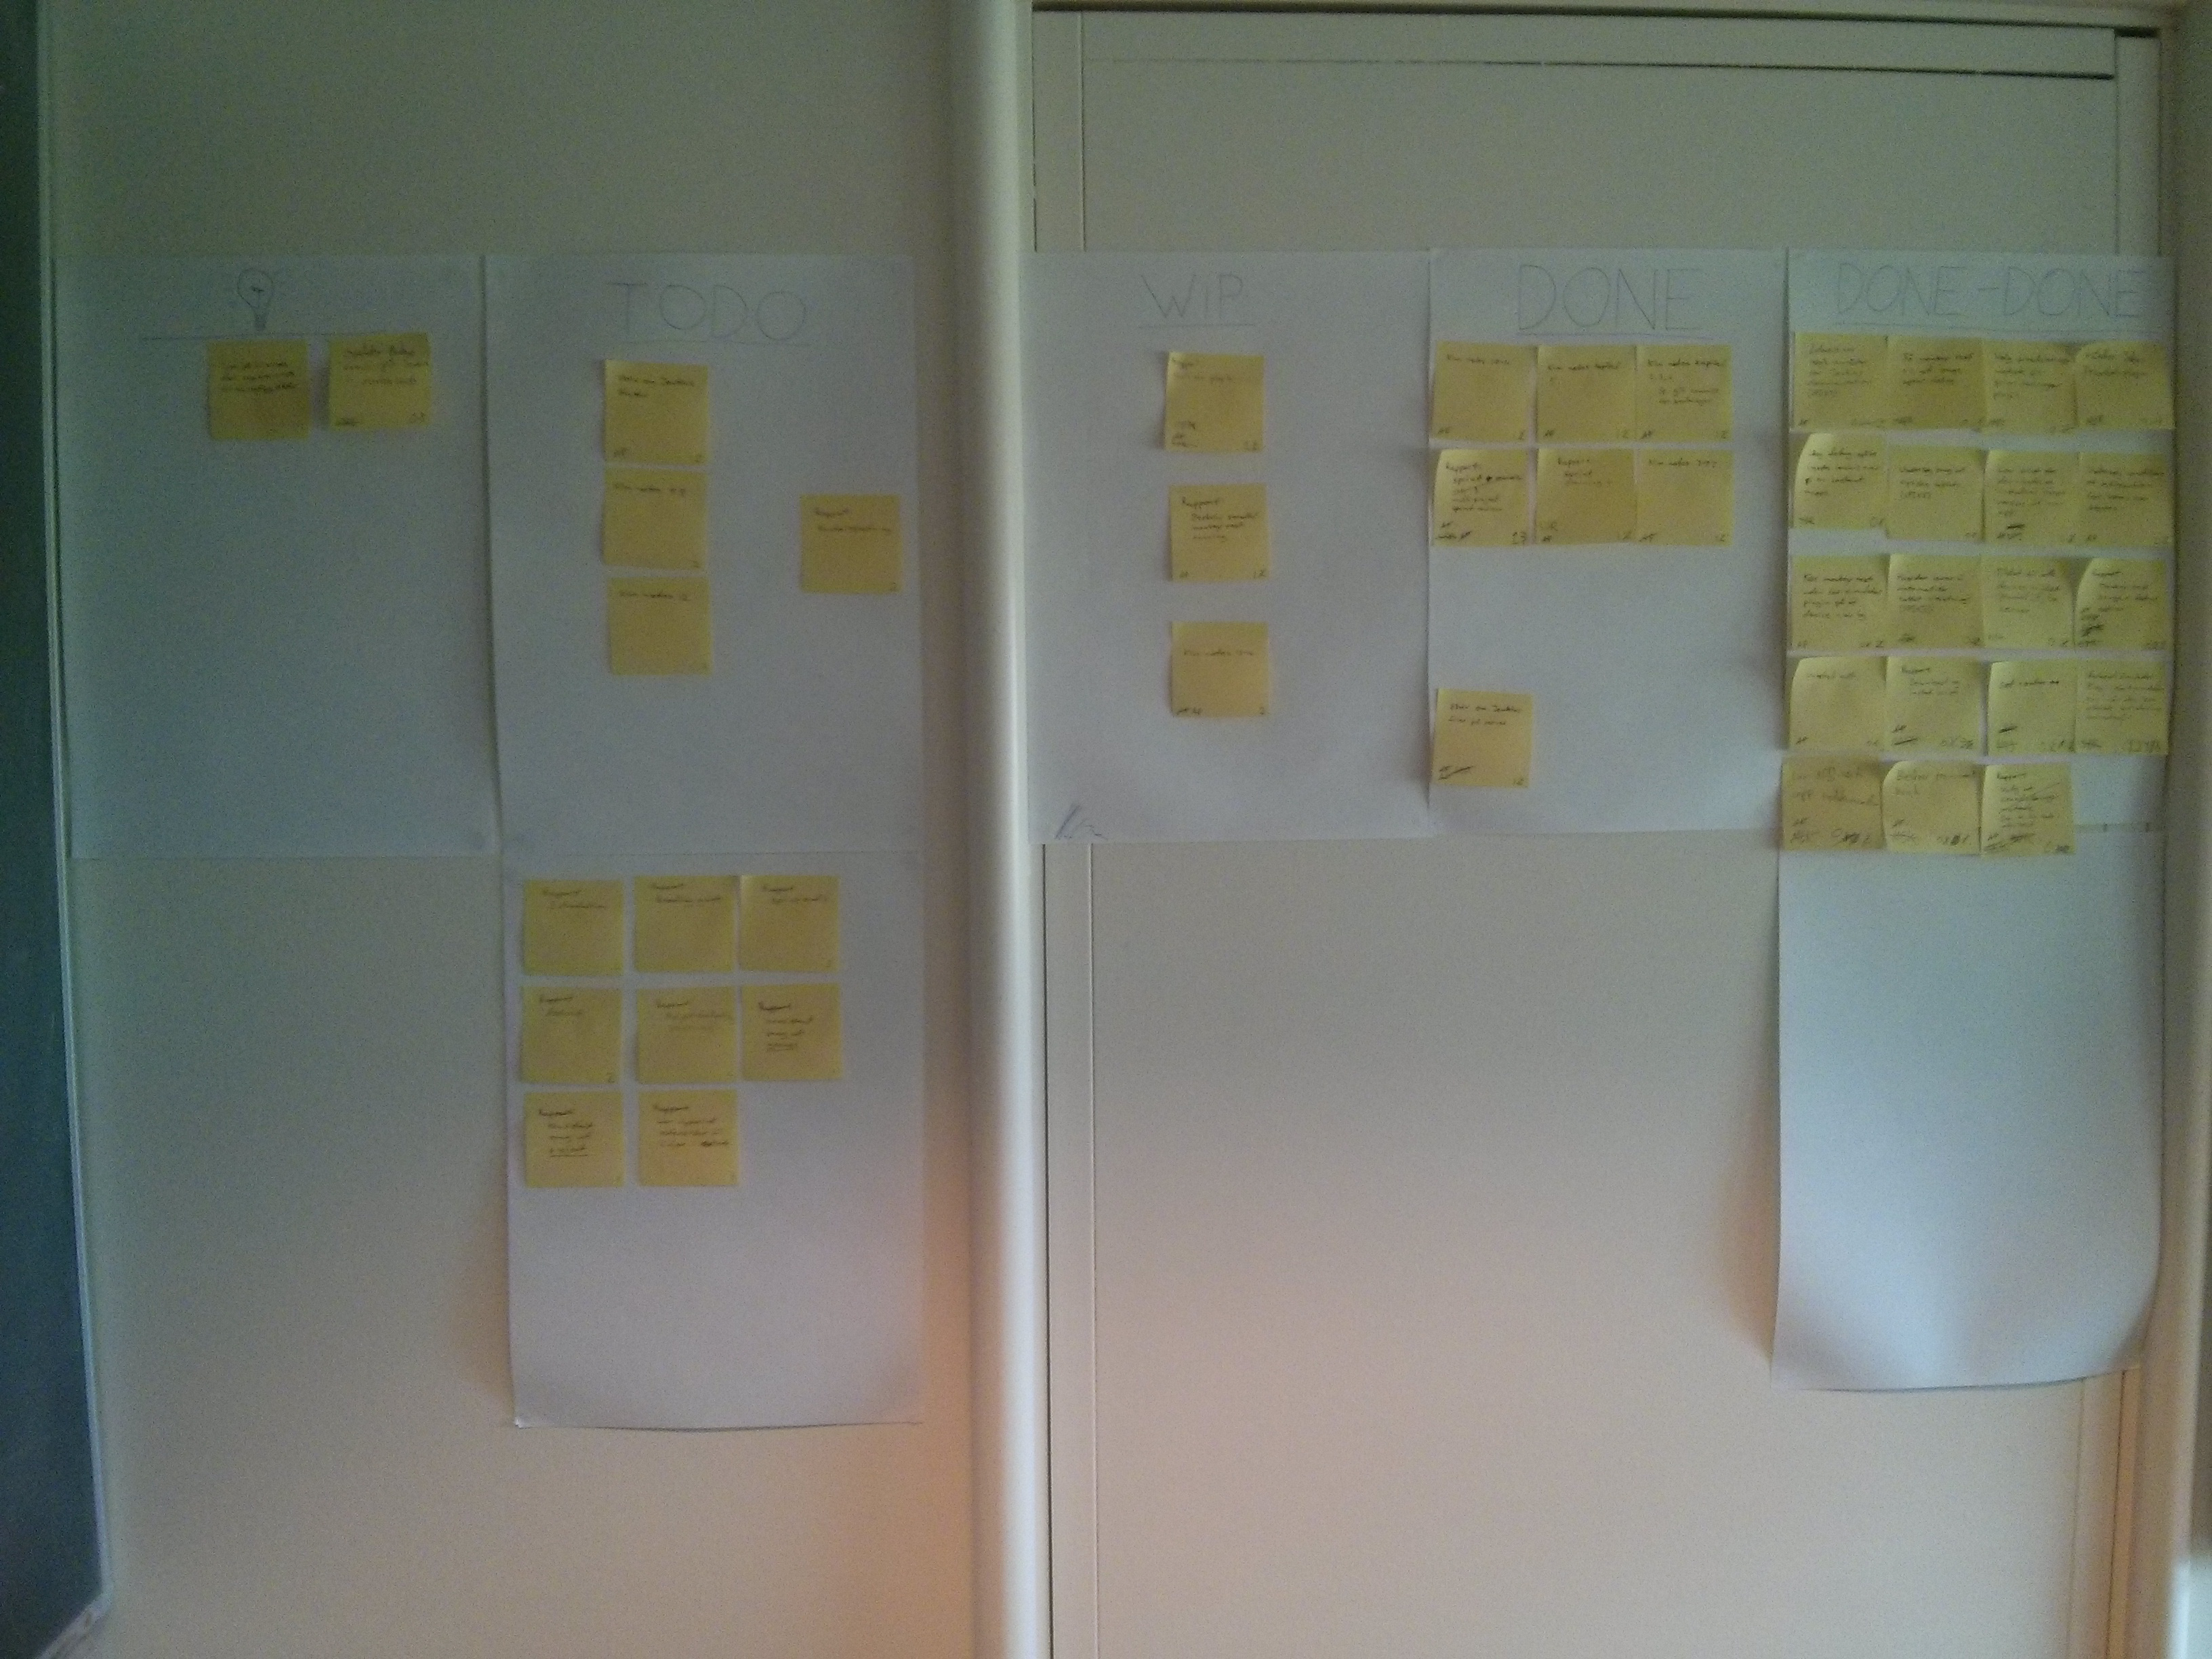
\includegraphics[width=0.49\textwidth]{kanban}

\end{frame}
\note{
	\begin{itemize}
		\item \textbf{Internt}: Valgt Scrum
    \item Det passer godt ind i multiprojektet.
    \item \textbf{Scrumboardet}: valgte backlog items > \textbf{opsplitning} i opgaver > \textbf{planning} poker. Enhed: \textbf{halvdage} (tidligere god erfaring)
    \item \textbf{Daily Scrum}
    \begin{itemize}
      \item Fortæller om \textbf{fremgang}, problemer, mm
      \item Vælger opgaver fra sprint backloggen
      \item Opdaterer \textbf{burndown}, visuel fremgang
    \end{itemize}

    \item På burndown: \textbf{Vi er bagefter}:
    \begin{itemize}
      \item Ideelle burndown, summerede resterende opgaver.
      \item \textbf{Prioriterer} resterende opgaver, \textbf{vigtigste fuldført}.
      \item Dette kan ses på scrumboardet. Nederste tasks er nedprioriterede.
    \end{itemize}
    
	\end{itemize}
}


%%%%%%%%%%%%%%%%%%%%%%%%%
%% SCM
%%%%%%%%%%%%%%%%%%%%%%%%%


\begin{frame}
    \frametitle{Continuous Integration}
    \begin{itemize}
      \item Automatisk testning af apps og biblioteker
      \item Hyppig merge med master branch
      \item Nyeste dokumentation
      \item Automatisk kørsel af statiske analyser
    \end{itemize}
\end{frame}
\note{
	\begin{itemize}
    \item CI \textbf{binder} tingene under konfigurationsstyring \textbf{sammen}.
    \item Gennemgå \textbf{bullets} på slides.
    \item[]
    \item \textbf{Agil}: giver \textbf{stort ansvar} til udviklerne.
    \item De \textbf{comitter direkte} til \textbf{master} branch, derfor skal de comitte \textbf{ofte}.
    \item Vi arbejder nemlig meget i de samme ting.
    \item[]
    \item Dette giver konstant \textbf{nye versioner}: skal konfig-styres.
    \item Alt i alt: \textbf{CI} er inde og \textbf{røre mange af tingene} under konfig-styring.
    \item Tingene kan siges at blive\textbf{ understøttet af CI}.
	\end{itemize}
}
\section[Job Flow]{Job Flow --- Long Title}

% Emneoverskrift. Start jeres del med denne:
\begin{frame}
  \frametitle{}
  \begin{center}
    {\Huge Job Flow}
  \end{center}
\end{frame}
\note{
  \begin{itemize}
		\item Notes...
  \end{itemize}
}

% Indhold:
\begin{frame}
    \frametitle{Some Slide Title}
    HUSK AT SKRIVE PÅ DANSK!\\
    The quality of the training data is determined by:
    \begin{itemize}
        \item The number of samples
        \item Variance
        \item The distribution of classification
    \end{itemize}
\end{frame}
\note{
	\begin{itemize}
		\item Notes...
	\end{itemize}
}
\section[Kortere byggetider]{Kortere byggetider}

% Emneoverskrift. Start jeres del med denne:
\begin{frame}
  \frametitle{}
  \begin{center}
    {\Huge Kortere byggetider}
  \end{center}
\end{frame}
\note{
  \begin{itemize}
		\item Overgang
  \end{itemize}
}

% Indhold:
\begin{frame}
    \frametitle{Biblioteker som binære filer}
	Git submoduler resulterer i:
    \begin{itemize}
        \item Overflødig kompilering og test af kode
        \item Kompleksitet i styring af dependencies
        \item Svært at kontrollerer hvor biblioteker bliver released
        \item Den samme dependency kan forekomme flere steder i hvert projekt
    \end{itemize}
\end{frame}
\note{
	\begin{itemize}
		\item Samarbejde med Git gruppe
	\end{itemize}
}

\begin{frame}
    \frametitle{Biblioteker som binære filer}
    Todo: figur med build tider (jeg kunne ikke finde ud af tikz...)
    Emulator tager stadig lang tid
\end{frame}
\note{
    \begin{itemize}
        \item Notes...
    \end{itemize}
}

\begin{frame}
    \frametitle{Test på fysiske enheder}
    Router setup
    \begin{itemize}
        \item Fast IP til tablet første gang der forbindes
        \item Automatisk tildeling af porte og port forwarding
        \item Web server med liste af tilsluttede enheder
    \end{itemize}
\end{frame}
\note{
    \begin{itemize}
        \item Notes...
    \end{itemize}
}

\begin{frame}
    \frametitle{Test på fysiske enheder}
    Konfigurering af Tablets
    \begin{itemize}
        \item Tablets har indbygget fjernstyring over WiFi
        \item Skal slås til hver gang en enhed startes --- app'en sørger for det
        \item Kræver root adgang
        \item Forhindre Monkey Test i at tilgå topbaren
        \item Mangler sikker frakobling
    \end{itemize}
\end{frame}
\note{
    \begin{itemize}
        \item Notes...
    \end{itemize}
}

\begin{frame}
    \frametitle{Test på fysiske enheder}
    Konfigurering af Jenkins platformen
    \begin{itemize}
        \item Tilføj et pre-build step der forbinder til enheder
        \item Modificerer emluator plugin'et til at kontrollere om der er forbundne enheder
        \item Køre test
        \item Afbryde forbindelsen igen
    \end{itemize}
\end{frame}
\note{
    \begin{itemize}
        \item Notes...
    \end{itemize}
}
\section[Monkey test]{Monkey test}
% Emneoverskrift. Start jeres del med denne:
\begin{frame}
  \frametitle{}
  \begin{center}
    {\Huge Monkey test}
  \end{center}
\end{frame}
\note{
  \begin{itemize}
    \item Notes...
  \end{itemize}
}

\begin{frame}
  \frametitle{Monkey test}
  \begin{itemize}
    \item Automatisk UI test
    \item Hvorfor køre monkey tests?
    \begin{itemize}
      \item Ingen UI tests
      \item Stort ønske af andre udviklerer
    \end{itemize}
  \end{itemize}
\end{frame}
\note{
  \begin{itemize}
    \item Notes...
  \end{itemize}
}

\begin{frame}
  \frametitle{Omskrivning af apps}
  \begin{itemize}
    \item code snippet...
  \end{itemize}
\end{frame}
\note{
  \begin{itemize}
    \item Notes...
  \end{itemize}
}

% \begin{javacode}
% if (ActivityManager.isUserAMonkey())
%   Helper h = new Helper(this);

%   guardianId = h.profilesHelper.getGuardians().get(0).getId();
% }
% \end{javacode}

\begin{frame}
  \frametitle{Monkey test flow}
  \begin{itemize}
    \item Tilslut til tablets
    \item Installer APK'er
    \item Kør Dummy Database Inserter app
    \item Block notification bar
    \item Kør monkey test
    \item Rappoter resultater
  \end{itemize}
\end{frame}
\note{
  \begin{itemize}
    \item Kør demo sammen
  \end{itemize}
}

\section[Konklusion]{Konklusion}

% Emneoverskrift. Start jeres del med denne:
\begin{frame}
  \frametitle{}
  \begin{center}
    {\Huge Konklusion}
  \end{center}
\end{frame}
\note{
  \begin{itemize}
    \item Notes...
  \end{itemize}
}

% Indhold:
\begin{frame}
  \frametitle{Konklusion}
  \begin{itemize}
    \item Opsætning af værktøjer til støtte af udviklingsmetode
    \item Intern udviklingsmetode
    \item GIRAF-udviklingsmetodeforberinger
    \item GIRAF har bedre grundlag
  \end{itemize}
\end{frame}
\note{
  \begin{itemize}
    \item Notes...
  \end{itemize}
}

% Indhold:
\begin{frame}
  \frametitle{Anbefaldinger}
  \begin{itemize}
    \item Ændr subprojektstruktur
    \item Automatisering 
    \begin{itemize}
      \item Script deployment
      \item Monkey test notifikationer
    \end{itemize}
    \item Sikkert tabletfraforbindelse
    \item Skriv tests
  \end{itemize}
\end{frame}
\note{
  \begin{itemize}
    \item Notes...
  \end{itemize}
}

\section*{}

\begin{frame}
  \frametitle{Overview}
  \tableofcontents
\end{frame}

\end{document}
